\begin{frame}
\frametitle{UCB1 Theorem on Regret Bound}
\begin{theorem}
For all $K > 1$, if policy UCB1 is run on K arms having arbitrary reward
distributions $P_{1}, . . . , P_{K}$ with support in $[0, 1]$, then its expected regret after any number $n$ plays is at most,
\begin{align*}
\mathbb{E}[R_n]\leq \sum_{i\in A}\dfrac{8\log n}{\Delta_{i}} + \sum_{i\in A}\Delta_{i}\bigg(1+\dfrac{\pi^{2}}{3}\bigg) 
\end{align*}
where $\mu_{1}, . . . , \mu_{K}$ are the expected values of $P_{1}, . . . , P_{K}$ .
\end{theorem}
\end{frame}

\begin{frame}
\frametitle{UCB1 Proof}
\begin{itemize}
\item<1-> The main goal is to bound the number of pulls ($T_i(n)$) of the sub-optimal arm $i$ till the $n$-th timestep.
\item<2-> So, we will assume that the $i$-th arm has been pulled atleast $\ell$ times and bound the probability of how many times it can be pulled after that.
\begin{align*}
T_{i}(n)&\leq \ell +\sum_{t=K+1}^{n}\lbrace I_t=i, T_i(t-1)\geq \ell\rbrace
\end{align*}
\item<3-> But, this is nothing but the probability that how many times after the $\ell$ pulls the UCB of $*$ is less than the UCB of $i$ which will have the highest UCB among all arms in $A$ to be selected,
\begin{align*}
T_{i}(n)&\leq \ell + \sum_{t=1}^{\infty}\sum_{s=1}^{t-1}\sum_{s_i =\ell}^{t-1}\lbrace \bar{X}_{s}^{*} + c_{t,s} \leq \bar{X}_{i,s_i} + c_{t,s_i} \rbrace
\end{align*}
\end{itemize}
\end{frame}

\begin{frame}
\frametitle{UCB1 Proof}
\begin{itemize}
\item<1-> The main argument lies in this, 
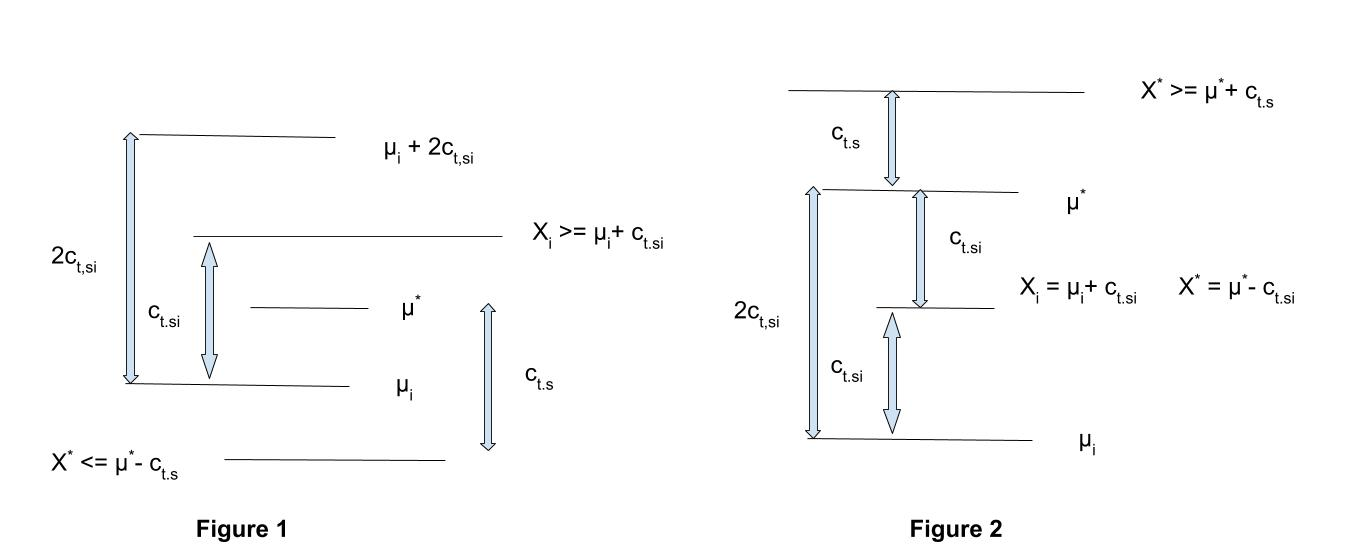
\includegraphics[scale=0.22]{img/UCB1_pic2} 
\item<1-> \begin{align*}
\bar{X}^{*}_{s}\leq \mu^* - c_{t,s};
\bar{X}_{i,s_i}\geq \mu_i + c_{t,s_i};
\mu^*  < \mu_i + 2c_{t,s_i}
\end{align*}
\end{itemize}
\end{frame}

\begin{frame}
\frametitle{UCB1 Proof}
\begin{itemize}
\item<0-> Now, we get the value of confidence interval $c_{t,s_i}=\sqrt{\dfrac{2\ln t}{s_i}}$ by plugging its value in the below equations,
\item<1-> $\mathbb{P}\lbrace  \bar{X}^{*}_{s}\leq \mu^* - c_{t,s}\rbrace\leq \exp\bigg(-2\big(\sqrt{\dfrac{2\ln t}{s}}\big)^2 s\bigg) \leq e^{-4\log t} \leq t^{-4}$
\item<2-> $\mathbb{P}\lbrace \bar{X}_{i,s_i} \geq \mu + c_{t,s_i}\rbrace\leq \exp\bigg(-2\big(\sqrt{\dfrac{2\ln t}{s_i}}\big)^2 s_i\bigg) \leq e^{-4\log t} \leq t^{-4}$
\item<3-> And by plugging $\ell=s_i =\bigg\lceil \dfrac{8\log n}{\Delta_{i}^{2}}\bigg\rceil$ in,
\begin{align*}
\mu^* - \mu_i - 2c_{t,s_i} = \mu^* - \mu_i - 2\sqrt{\dfrac{2\log t}{s_i}} \geq \mu^* - \mu_i -\Delta_i =0
\end{align*} 
we get $\mu^* - \mu_i - 2c_{t,s_i} \geq 0$. So for any pulls greater than $\ell$, $\mu^*$ will surely be atleast $2c_{t,s_i}$  more than $\mu_i$ and one of the rest two events will occur with high probability.
\end{itemize}
\end{frame}

\begin{frame}
\frametitle{UCB1 Proof}
\begin{itemize}
\item<1-> Summing everything up, any sub-optimal arm $i$ will get pulled atleast $\ell$ times and then the two events $\bar{X}^{*}_{s}\leq \mu^* - c_{t,s}$ and $\bar{X}_{i,s_i}\geq \mu + c_{t,s_i}$ will occur with atmost $t^{-4}$ probability.
\item<2-> \begin{align*}
\mathbb{E}[T_{i}(n)]&\leq \bigg\lceil \dfrac{8\log n}{\Delta_{i}^{2}}\bigg\rceil + \sum_{t=1}^{\infty}\sum_{s=1}^{t-1}\sum_{s_i =\ell}^{t-1}2t^{-4}\\
&\leq \dfrac{8\log n}{\Delta_{i}^{2}} +1 + \dfrac{\pi^{2}}{3}, \text{by Bazel's equation}
\end{align*}
\item<3-> So finally the cumulative regret is,
\begin{align*}
\mathbb{E}[R_n]&\leq \sum_{i\in A}\mathbb{E}[T_i (n)]\Delta_i
\leq \sum_{i\in A}\dfrac{8\log n}{\Delta_{i}} + \sum_{i\in A}\Delta_{i}\bigg(1 + \dfrac{\pi^{2}}{3}\bigg)
\end{align*}
\end{itemize}
\end{frame}